
\documentclass{article}
\usepackage[polish]{babel}
\usepackage[T1]{fontenc}
\usepackage[utf8]{inputenc}
\usepackage{textcomp,gensymb}
\usepackage{url}
\usepackage[breaklinks,hidelinks]{hyperref}
\usepackage{natbib}
\usepackage{graphicx}
\usepackage{geometry}
	\geometry{a4paper,total={170mm,257mm},inner=30mm,outer=20mm}
\usepackage{soul, color}
\usepackage{mathtools}
\usepackage{subcaption}
\usepackage{float}
\usepackage{titlesec}
\usepackage[colorinlistoftodos]{todonotes}
\graphicspath{ {/home/zby/MAGISTERKA/MGR/} }

\title{Grupowanie dokumentów}
\author{inż. Zbigniew Manasterski \\[15pt]\footnotesize Promotor: mgr inż. Rajmund Kożuszek}


\newfloat{maths}{h}{zma}
\floatname{maths}{Formuła}

\newcommand{\sectionbreak}{\clearpage}

\newcommand{\needspace}[1]{%
	\begingroup
	\setlength{\dimen@}{#1}%
	\vskip\z@\@plus\dimen@
	\penalty -100\vskip\z@\@plus -\dimen@
	\vskip\dimen@
	\penalty 9999%
	\vskip -\dimen@
	\vskip\z@skip % hide the previous |\vskip| from |\addvspace|
	\endgroup
}

\newcommand{\myparagraph}[1]{\paragraph{#1}\mbox{}\\}
\newcommand{\mysubsection}[1]{\needspace{5\baselineskip}}
\newcommand{\mysubsubsection}[1]{\needspace{5\baselineskip}}

\begin{document}

\linespread{1.5}\selectfont

\renewcommand{\labelenumii}{\theenumii}
\renewcommand{\theenumii}{\theenumi.\arabic{enumii}.}
\maketitle

\newpage
\tableofcontents
\newpage

\section{Wstęp}
Obecnie informacja jest bardzo łatwo dostępnym towarem. Wykorzystując Internet, można znaleźć wiele dokumentów, filmów i muzyki, mniej lub bardziej interesujące dla potencjalnego odbiorcy. Ilość dostępnej informacji jest przytłaczająca i bardzo trudno dokonać poprawnej selekcji informacji, rozumianej jako dobór takich danych, które są faktycznie pożądane przez odbiorcę. W celu rozwiązania takich problemów zaczęły powstawać serwisy, które na podstawie muzycznych, filmowych czy książkowych kategorii, automatycznie proponowały użytkownikom nowe, pasujące do ich upodobań, utwory – pochodzące z tej samej kategorii, do której wcześniej już użytkownik sięgał. W takim podejściu, użytkownicy są obiektami otrzymującymi pewne etykiety na podstawie skonsumowanej treści – każdy użytkownik jest przydzielany do pewnej kategorii. Zbiór informacji o utworach po jakie użytkownik sięgał jest cechą danego użytkownika. Wadą tego procesu jest to, że treści, które nie dotrą do przynajmniej jednego użytkownika, nie będą dostępne dla żadnego z nich.

Drugim podejściem do problemu selekcji informacji jest umożliwienie użytkownikowi jej przeglądania za pomocą wzorca/klucza lub przykładu. Wzór może się ograniczać do pewnego zbioru podstawowych elementów, składających się razem na informację – na przykład słów. Rezultaty takiego podejścia mogą być bardzo niezadowalające, ponieważ – w zależności od zbioru danych w którym prowadzone jest przeglądanie – wyniki mogą zawierać treści tylko luźno powiązane z zadanym zbiorem. Dodatkowo, klucz może być użyty w kontekście różnym od takiego, jaki jest poszukiwany przez użytkownika. W podejściu tym istotna staje się konstrukcja zbioru informacji. Powinna ona dzielić możliwe rozległy zbiór informacji na odpowiednio małe grupy obiektów, które są do siebie podobne. Wtedy rozpoczynając przeglądanie od interesującego obiektu, otrzymuje się łatwy dostęp do innych obiektów z jego grupy, które mogą nas potencjalnie zainteresować.

Pierwsze podejście do selekcjonowania i wyszukiwania informacji zaprezentowane w tym rozdziale nazywane jest klasyfikacją informacji. Nowych użytkowników serwisu muzycznego oznaczamy etykietą 'rock' jeżeli słucha muzyki rockowej, nie tworzymy nowych etykiet (grup), pozwalamy co najwyżej na kilka przyporządkowań jednego użytkownika do różnych etykiet. 

Druga metoda nazywana jest grupowaniem – jest to nienadzorowany proces podziału wzorców (obserwacji, danych, wektorów cech) na grupy (klastry). Stosując grupowanie na całym zbiorze użytkowników serwisu muzycznego można odkryć, że osoby słuchające muzyki jazzowej oraz rockowej często lubią słuchać również bluesa. Na podstawie tak dobranych grup obiektów, (obiektem jest zbiór odsłuchiwanej przez użytkownika muzyki) inni użytkownicy mogliby odkryć utwory spoza ich ulubionego gatunku muzycznego, które również by im się spodobały.  Przedmiotem tej pracy będzie wyłącznie grupowanie, sposoby jego przyspieszenia oraz usprawnienia. Podjęta zostanie próba zdefiniowania takiego procesu grupowania, który da wyniki podobne do takich, jakie byłyby wynikiem ręcznego grupowania wykonanego przez użytkownika. Praca ograniczona będzie jedynie do analizy problemu grupowania dokumentów.
Zaproponowany zostanie relatywnie nowy sposób wykorzystania algorytmu minimalnego drzewa rozpinającego do wyznaczenia podziału początkowego przy grupowaniu danych tekstowych. Omówiony będzie również współczynnik często używany do grupowania takich danych, jego zależność od wariancji występowania słów w zbiorze dokumentów oraz sposób, w jaki można to wykorzystać do przyspieszenia grupowania.

\newpage
\section{Podstawy grupowania}

Wszystkie rodzaje grupowania mają pewne wspólne zagadnienia. Trzeba wybrać miarę podobieństwa odpowiednią dla używanych danych - szybką i dającą jednoznaczne wyniki. Następnie wykonać kilka kroków przygotowawczych i po zakończonym grupowaniu, jego wyniki powinny być ocenione. Wszystkie powyższe zagadnienia są przybliżone w tym rozdziale.

\subsection{Zadania obejmujące grupowanie}
Proces grupowania składa się z kilku kroków wspólnych dla wszystkich tych algorytmów [1].
\begin{enumerate}
	\item Wybór sposobu reprezentacji obiektów.
	\item Wybór parametrów takich jak:
	\begin{itemize}
		\item liczba grup, do których dane będą przydzielane;
		\item istotne cechy obiektów.
	\end{itemize}
	\item Określenie miary podobieństwa odpowiedniej dla rodzaju porównywanych danych.
	\item Wykonanie grupowania.
	\item Stworzenie zwięzłej i prostej (dla człowieka, albo dla programu – w zależności od celu wykonywania grupowania) reprezentacji wyjściowych zbiorów danych.
	\item Dokonanie oceny wyników grupowania.
\end{enumerate}

Sposób reprezentacji obiektu odnosi się do sposobu opisu cech obiektu – reprezentacji liczbowej lub słownej, dziedziny, metody wyznaczenia wartości tych cech (na przykład momenty kształtu opisujące obiekty na obrazie).

Wybór cech obiektu może polegać na wyborze cech o najmniejszej wzajemnej korelacji, takich co do których wiadomo, że dają dobre wyniki grupowania przy określonym rodzaju algorytmu. Można również stworzyć nowe cechy na podstawie już istniejących, co może ułatwić i przyspieszyć porównywanie, pod warunkiem, że umiemy odpowiednio odwzorować kombinację dwóch lub więcej cech do nowej dziedziny. Dodatkowo, wybierając cechy do użycia podczas  grupowania, należy pamiętać o tym, że każda cecha to dodatkowy wymiar, który musi znaleźć się na wejściu funkcji obliczającej podobieństwo obiektów. Im mniej cech, tym większą szybkość będą miały algorytmy wrażliwe na liczbę wymiarów, jednocześnie wyniki grupowania mogą być trochę gorsze, bo z każdą odrzuconą cechą tracimy informacje o porównywanych obiektach.


\subsection{Miara podobieństwa}
Jest to najczęściej funkcja odległości pomiędzy dwoma obiektami. Jest wiele różnych funkcji odległości, z których najpopularniejsza jest odległość Euklidesowa (stanowiąca szczególny przypadek odległości Minkowskiego dla liczby wymiarów równej 2)\todo{Czy numerować wzory? Jak nazwać? Formuła, Wyrażenie, Wzór}.

\begin{maths}
	\centering
	\[(\sum_{k=1}^{d} |x_{i,j} - y_{i,j}|^p)^\frac{1}{p}\]
	\caption{Odległość Minkowskiego}
	\label{mth:minkowski}
\end{maths}


Inną miarą odległości pomiędzy dwoma wektorami liczbowymi jest miara Mahalanobisa, wyrażona wzorem:

\[\delta(x_{i}, x_{j}) = \sqrt{(x_{i} - x_{j})C^{-1}(x_{i} - x_{j})^T} \]
gdzie C to macierz kowariancji mająca odzwierciedlać charakter klasy punktów.

Podane powyżej przykłady miar są mało złożone. Takie funkcje można dodatkowo skomplikować i ulepszyć uwzględniając kontekst, czyli najbliższe otoczenie badanego obiektu. W zależności od kontekstu mogą zmienić się wartości opisujące tylko niektóre lub wszystkie cechy obiektu (kontekst nie musi dotyczyć wszystkich cech obiektu). Uwzględnienie kontekstu zwykle pozwala poprawić wyniki grupowania, jednak powoduje dodatkowy narzut obliczeniowy – porównywanie obiektów staje się bardziej kosztowne. Wprowadza również nowe problemy: jak szeroki kontekst brać pod uwagę, z jakimi wagami i dla jakich cech go uwzględniać. Odpowiedzi na te pytania można znaleźć wykonując eksperymenty – badając wyniki grupowania dla różnych wariantów i określając, które grupowanie dało lepsze wyniki (problem ocen wyników grupowania będzie poruszony w dalszej części pracy).

Kolejną możliwością porównywania obiektów jest zdefiniowanie dodatkowych, abstrakcyjnych kryteriów zależnych na przykład od globalnego kontekstu. Grupując punkty na płaszczyźnie można zwracać uwagę jedynie na ich odległości od siebie, ale można wykorzystać inne kryterium – punkty są do siebie podobne, jeżeli są częścią obwiedni tej samej figury geometrycznej. W takim przypadku należy najpierw określić, jakie figury są brane pod uwagę, oraz przeprowadzić wyszukiwanie tych figur w zbiorze danych. Takie podejście daje praktycznie nieograniczone możliwości grupowania treści, pomimo wprowadzenia dodatkowych kosztów obliczeniowych.

\subsection{Ocena wyników grupowania}

Wyniki grupowania stanowią obiekty przydzielone do różnych zbiorów. Jeżeli w warunkach początkowych znalazły się parametry określające zbiory wyjściowe, to może się zdarzyć, że do niektórych z nich nie zostaną przydzielone żadne obiekty, albo że wszystkie obiekty będą przydzielone do jednego zbioru. Oba powyższe warianty wyników mogą być poprawne i pożądane. Aby to ocenić można próbować porównać uzyskane wyniki z wynikami otrzymywanymi za pomocą znanych implementacji podobnych algorytmów grupowania. Można też postawić pytanie, czy wyniki grupowana spełniają cel, który użytkownik chciał osiągnąć. Stwierdzenie czy możliwa jest łatwiejsza selekcja informacji wymaga przeprowadzenia eksperymentów na reprezentatywnej grupie potencjalnych odbiorców selekcjonowanych treści.

Jeżeli do grupowania zostały użyte metody oparte na statystyce, walidację wyników można wykonać tylko stosując odpowiednio dobrane metody analizy statystycznej [odniesienie do Jain 1.2, 5str]

Wyniki grupowania można oceniać ze względu na jakość przydziału obiektów do grup. Jeżeli w którejś z grup znajdują się obiekty znacznie odległe od siebie nawzajem, ale jednocześnie spokrewnione ze sobą, poprzez łańcuch podobieństw z innymi obiektami z tego zbioru, to mamy do czynienia z efektem łańcuchowym – błędem grupowania spowodowanym złym dobraniem algorytmu lub kryterium podobieństwa.

Do oceny grupowania stosuje się różnego rodzaju miary jakości grupowania. Jednym z najbardziej popularnych wskaźników jest miara Silhouette [5], wyrażona wzorem:

\[s(i) = \frac{b(i) - a(i)}{max|a(i),b(i)|}\]

Gdzie współczynniki a oraz b, to:

\begin{itemize}
	\item a(i) - średnia odległość pomiędzie obiektem i, a jego sąsiadami z grupy,
	\item b(i) – najmniejsza średnia odległość pomiędzy obiektem i, a obiektami z innej grupy (nazywanej grupą sąsiadującą).
\end{itemize}
Parametry te można obliczyć dla jednej z grup lub całego zbioru. Średnie s(i)  dla jednej grupy określają jej gęstość, natomiast średnie s(i) obliczone dla całego analizowanego zbioru danych określają jakość grupowania.

Wartości s(i) zmieniają się od -1 do 1. Jeżeli wartość jest bliżej -1 oznacza to, że element i powinien być zakwalifikowany do grupy sąsiadującej. Jeżeli wartość s(i) znajduje się bliżej 1, oznacza to, że obiekt i został poprawnie zgrupowany. Natomiast jeżeli wartość s(i) znajduje się w pobliżu  0, oznacza to, że obiekt i znajduje się na granicy dwóch odpowiednich dla niego grup (odrobinę powyżej zera – obiekt jest w lepszej grupie, odrobinę poniżej zera – obiekt jest w gorszej grupie).

Rezultaty działania algorytmu grupowania mogą być również poddane ocenie poprzez porównanie ich, z wynikami grupowania wykonanego przez człowieka. Załóżmy, że danymi wejściowymi jest zbiór artykułów prezentowanych na konferencjach naukowych. Prezentacje zostały przez organizatorów (na podstawie znajomości treści lub abstraktów artykułów, recenzji, deklaracji autorów) podzielone na sekcje tematyczne. Być może algorytm przeprowadzający grupowanie powinien podzielić te artykuły na takie same grupy. Jednak należy pamiętać o tym, że podział wykonany przez człowieka nie musiał być najlepszym możliwym. 

Przykładem na niedoskonałą ocenę człowieka są różnice, jakie występują przy doborze tagów dla dokumentów. Twórcy artykułów często oznaczają je słowami kluczowymi, które stosunkowo rzadko występują w tekście. Czytelnicy – wolontariusze, którzy mieli za zadanie oznaczać przeglądane materiały najczęściej dobierali inne zestawy słów kluczowych, ze zbioru takich słów, które częściej występowały w tekście. [Potrzebne dobre uzasadnienie w bibliografii].

\newpage
\section{Rodzaje grupowania}

Algorytmy grupowania można podzielić na kilka kategorii, ze względu na ich sposób działania. Wyróżnia się następujące sposoby działania algorytmów grupowania:

\begin{enumerate}
	\item Agregujące – dzielące: Algorytmy sumujące traktują początkowe dane jako zestaw zbiorów jednoelementowych i na podstawie zadanego kryterium łączą mniejsze zbiory w większe, dopóki nie zostanie osiągnięty warunek zakończenia (odpowiednia liczba zbiorów końcowych, oraz średnia liczność elementów w zbiorach, w aktualnej iteracji). Algorytmy dzielące przyjmują założenie, że dane początkowe, to jeden zbiór zawierający wszystkie obiekty. Zbiór ten jest dzielony na mniejsze według zadanego kryterium, którym może być na przykład średnia odległość grupy obiektów od pozostałych. Algorytm kończy się jeżeli osiągnie założone warunki podziału, podobnie jak w przypadku algorytmów agregujących.
	\item Sekwencyjne – równoległe: W algorytmach typu sekwencyjnego każda cecha porównywana jest osobno – np. najpierw porównywane są współrzędne X punktu, a dopiero później współrzędne Y. Przy bardziej skomplikowanych wektorach cech może to prowadzić do gorszych wyników grupowania obiektów. Niektóre z algorytmów grupowania działające tą metodą w wyniku potrafią dać 2d grup, gdzie d jest liczbą wymiarów \todo{jain 5, 11str}. Przeciwnym podejściem do takiego grupowania jest grupowanie równoległe. Wiele lub wszystkie cechy porównywanych obiektów są jednocześnie brane pod uwagę – wzrasta minimalnie koszt obliczeniowy.
	\item Dokładne – rozmyte: W grupowaniu dokładnym każdy obiekt jest przypisywany  do co najwyżej jednego zbioru (może być niesklasyfikowany, potraktowany jako szum, jeżeli nie mieści się w żadnym z przyjętych na początku zbiorów – kategorii obiektów). W grupowaniu rozmytym każdy obiekt może zostać przypisany do więcej niż jednego zbioru. Prezentacja wyników może być wtedy trochę bardziej złożona, ale za to wyniki grupowania mogą dokładniej odzwierciedlać rzeczywistość – rzadko da się przydzielić jakąś treść tylko do jednej kategorii.
	\item Deterministyczne – stochastyczne: Algorytmy deterministyczne dla określonych warunków początkowych i danych wejściowych zwrócą zawsze takie same wyniki. Stochastyczne wprowadzają element losowości do swojego działania, dlatego kilkukrotne uruchomienie takiego algorytmu dla tych samych danych wejściowych i warunków początkowych może dać różne wyniki.
	\item Przyrostowe – nieprzyrostowe: Różnica między tymi dwoma typami grupowania polega na wykorzystaniu cech obiektów podczas grupowania. W przypadku podejścia przyrostowego, algorytm grupujący nie porównywał obiektów przy użyciu ich wszystkich cech jednocześnie - tylko używał określonych cech w kolejnych iteracjach. Podejście to wynikało z ograniczeń jakie kiedyś nakładał dostępny sprzęt komputerowy. Obecnie używa się raczej algorytmów nieprzyrostowych - które przy porównywaniu obiektów zawsze biorą pod uwagę wszystkie ich cechy. 
\end{enumerate}

\subsection{Grupowanie hierarchiczne} 
\label{subsec:grupHier}
Algorytmy grupowania, które produkują drzewo podziałów, nazywane są hierarchicznymi. W tego typu implementacjach grupowania użytkownik ma komfort pobrania podziału z dowolnego poziomu drzewa, na podstawie kryterium liczebności liści pod pobieranymi węzłami. Zwykle korzeniem takiego drzewa jest zbiór zawierający wszystkie elementy, a jego liśćmi są zbiory jednoelementowe, po jednym dla każdego obiektu, który znajdował się w zbiorze wejściowych danych.

Grupowanie hierarchiczne można podzielić na dwa podtypy:

\begin{enumerate}
	\item Z wiązaniem pojedynczym (ang. \textit{single link}):
	Do określania przynależności obiektu do zbioru (podobieństwa) używana jest najmniejsza odległość pomiędzy badanym obiektem, a obiektem znajdującym się w analizowanym zbiorze. Podejście takie umożliwia powstanie efektu łańcuchowego – niepoprawnego podziału obiektów na grupy.
	\item Z wiązaniem pełnym (ang. \textit{complete link}): 
	W przeciwieństwie do wiązania pojedynczego, tutaj brana jest pod uwagę największa odległość pomiędzy obiektem, a innym obiektem z badanej grupy. Wyklucza to możliwość powstania efektu łańcuchowego. Wyniki grupowania algorytmami tego typu są zwykle zbiorami gęstymi.
\end{enumerate}

Analizując rezultaty algorytmów stosujących wiązanie pojedyncze można stwierdzić, że często dają grupy, które są poszarpane i wydłużone. Jednocześnie takie algorytmy są uznawane za bardziej wszechstronne, działające lepiej na nietypowych zbiorach danych \todo{jain, 5.1, 13, rysunek}, na których zastosowanie działania z wiązaniem pełnym nie przyniosłoby oczekiwanych rezultatów. Mimo tej zalety, uznaje się na podstawie wielu obserwacji \todo{jain}, że generalnie lepiej jest używać wiązania pełnego, daje ono zwykle lepsze, bardziej zwarte i użyteczne wyniki grupowania.

Algorytmy hierarchiczne są bardziej uniwersalne od algorytmów partycjonujących.\todo{jain before 5.2} Wersja z wiązaniem pojedynczym działa dobrze dla danych nie-izotropowych, rozłącznych, łańcuchowych, lub też podzielonych na rozłączne skoncentrowane grupy. Natomiast typowy algorytm grupowania partycjonującego taki jak k-średnich działa dobrze tylko dla danych izotropowych – regularnych. Jednak trzeba zaznaczyć, że zwykle złożoność obliczeniowa i pamięciowa algorytmów partycjonujących jest mniejsza od złożoności algorytmów grupowania hierarchicznego. Jednocześnie jest możliwe zaprojektowanie algorytmu hybrydowego wykorzystującego zalety obu tych sposobów grupowania. \todo{Bibliografia, przed 5.2, jain Murty and Krishna 1980}

\subsubsection{Przykłady algorytmów grupowania hierarchicznego}

W tym rozdziale zaprezentowane zostaną przykładowe algorytmy grupowania hierarchicznego, z różnymi wiązaniami, działające agregująco. 

\myparagraph{Algorytm grupowania z wiązaniem pojedynczym}

Działanie takiego algorytmu, działającego na zasadzie agregacji zbiorów można przedstawić za pomocą następujących kroków.

\begin{itemize}
	\item Umieść każdy obiekt w odrębnej, jednoelementowej grupie. Utwórz listę odległości pomiędzy wszystkimi parami obiektów i posortuj ją rosnąco.
	\item Przejdź przez elementy posortowanej listy tworząc graf dla każdej unikatowej wartości dk (odległości pomiędzy k-tą parą na liście). Wierzchołkami tego grafu są obiekty, które są połączone krawędzią, jeżeli odległość pomiędzy nimi jest mniejsza niż dk. Ten krok jest powtarzany dopóki wszystkie obiekty nie znajdą się w grafie.
	\item Na wyjściu algorytmu otrzymywana jest zagnieżdżona hierarcha grafów, którą można przeciąć na dowolnym poziomie i tak uzyskanego podziału, używać jako wyniku grupowania.
\end{itemize}

Odległość pomiędzy dwoma grupami, które są liczniejsze niż jednoelementowe, jest obliczana według metody wiązania pojedynczego. Jest to najmniejsza odległość pomiędzy parą obiektów z tych grup, tak jak jest to opisane w rozdziale \ref{subsec:grupHier}. Na rysunku \ref{fig:grupHPng} można zaobserwować wady tego algorytmu - obecność efektu łańcuchowego w wynikach grupowania.

\begin{figure}[H]
	\centering
	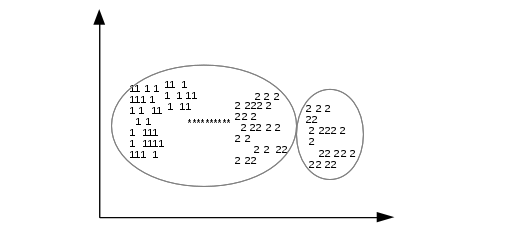
\includegraphics[scale=0.9]{hierarchiczneGrupowanie.png}
	\caption{Wyniki grupowania obiektów za pomocą algorytmu hierarchicznego z wiązaniem pojedynczym - 1 i 2 to dwa rodzaje obiektów, * to obiekty stanowiące szum, łączące oba zbiory. Obwódkami zakreślone są powstałe grupy.}
	\label{fig:grupHPng}
\end{figure}

\myparagraph{Alogrytmy grupowania z wiązaniem pełnym}

Kroki tego algorytmu wyglądają identycznie jak algorytmu opisanego powyżej. Różnicę pomiędzy nimi stanowi sposób określania odległości pomiędzy dwoma grupami. Jest ona wyznaczana na podstawie największej odległości pomiędzy dwoma obiektami z porównywanych grup, tak jak zostało to opisane w rozdziale \ref{subsec:grupHier}. Mimo, że jest to jedyna różnica, wyraźnie ona wpływa na jakość uzyskiwanych wyników, co widać na rysunku \ref{fig:grupHChain}.

\begin{figure}[H] 
	\centering
	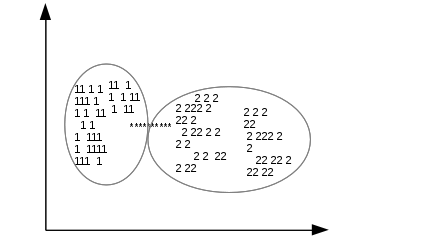
\includegraphics[scale=0.9]{grupHChain.png}
	\caption{Wyniki grupowania obiektów za pomocą algorytmu hierarchicznego z wiązaniem pełnym - 1 i 2 to dwa rodzaje obiektów, * to obiekty stanowiące szum, łączące oba zbiory. Obwódkami zakreślone są powstałe grupy.}
	\label{fig:grupHChain}
\end{figure}

\myparagraph{Grupowanie hierarchiczne i agregujące z wiązaniem pełnym}

Kroki tego algorytmu wyglądają podobnie do obu opisanych powyżej, jednak różnią się tym, że każdą nowo powstałą grupę dodajemy do listy dystansów pomiędzy grupami:
\begin{itemize}
	\item Oblicz macierz odległości między wszystkimi parami obiektów – każdy obiekt jest jednoelementową grupą.
	\item Znajdź dwie najbardziej podobne do siebie grupy i złącz je w jedną grupę. Uaktualnij macierz odległości tak, żeby odzwierciedlała tą operację.
	\item Zakończ algorytm jeżeli wszystkie obiekty znajdują się w jednej grupie.
\end{itemize}

Dodatkowo nie zajmujemy się ponownie raz złączonymi obiektami, w przeciwieństwie do tego jak było we wcześniej opisanych algorytmach.

W zależności od sposobu aktualizacji macierzy odległości w drugim kroku (obliczenia dystansu pomiędzy grupami, ewentualne ustalenie środka nowej grupy) można stworzyć różne wersje grupowania agregującego, hierarchicznego. Implementacja algorytmu dzielącego wyglądałaby bardzo podobnie – tylko rozpoczynałby on od grupy zawierającej wszystkie obiekty i dzielił je na dwie grupy wybierając obiekty do każdej z grup na podstawie jakiegoś zadanego kryterium. \todo{Odniesienie do jain – ewentualnie dać jedno na cały podrozdział}

\subsection{Grupowanie partycjonujące}
Ten sposób grupowania daje w wyniku pojedynczy podział obiektów na grupy. Nie są tworzone skomplikowane struktury takie jak drzewa/grafy podziałów opisywane w rozdziale 2.1.1. Dzięki temu takie podejście jest dobre szczególnie wtedy, kiedy algorytm ma działać na dużych, złożonych zbiorach danych – jest mniej czasochłonne, a wyniki zajmują mniej pamięci. Problemem związanym z zastosowaniem takiego sposobu grupowania danych jest wybór pożądanej liczby grup wyjściowych, jednak istnieją opracowania zawierające opis rozwiązaniu pozwalającego pomóc w doborze tego parametru. \todo{Dubes 1987 – from jain 5.2}
 
Techniki partycjonujące najczęściej tworzą podziały wynikowe poprzez optymalizowanie kryterium, będącego jakiegoś rodzaju funkcją odległości. Kryterium to może być zdefiniowane lokalnie (dotyczyć tylko pewnego wybranego podzbioru obiektów) albo globalnie (dotyczyć wszystkich obiektów w przetwarzanym zbiorze danych). Kombinatoryczne poszukiwanie zbioru możliwych podziałów dla optymalnej wartości kryterium jest obliczeniowo bardzo złożone. Dlatego w praktyce algorytm wykonywany jest wielokrotnie dla różnych podziałów początkowych (np. uzyskanych po poprzednich przebiegach) i kończony jest gdy podział osiągnie pewną założoną wartość kryterium. Jeżeli kryterium było zdefiniowane lokalnie (np. odległość od punktu do centrów grup – reprezentujących tylko zbiory punktów) warunkiem zakończenia algorytmu może  być również brak zmian w podziale obiektów pomiędzy grupami. Często w implementacjach takich algorytmów warunkiem początkowym jest istnienie początkowej struktury podziałów – czasami jest ona budowana heurystycznie na początku algorytmu. 

Najpopularniejszym kryterium wykorzystywanym do określenia błędu podziału jest błąd kwadratowy, wyrażony wzorem:

\[ e^2(H,L) = \sum_{j=1}^{K}\sum_{i=1}^{n_{j}}||x_{i}^j - c_{j}||^2 \]
Gdzie c to średni element w zbiorze j a $x_{i}$ to i-ty element tego zbioru.

\subsubsection{Przykłady algorytmów partycjonujących}

W tym rozdziale zaprezentowane zostaną przykładowe algorytmy partycjonujące. Do najpopularniejszych należą algorytmy k-średnich oraz błędu kwadratowego.

\myparagraph{Algorytm k-środków/średnich}
Najczęściej stosowanym algorytmem typu partycjonującego jest algorytm k-środków. Jego kolejne kroki można przedstawić w następujący sposób:
\begin{itemize}
	\item Wybierz k grup i k środków powiązanych z k losowo wybranymi obiektami lub losowo utworzonymi punktami znajdującymi się wewnątrz dziedziny przestrzeni opisującej cechy wszystkich obiektów.
	\item Przypisz każdy obiekt do najbliższego środka grupy.
	\item Oblicz nowe współrzędna środków grupy na podstawie przynależności obiektów do danej grupy. 
	\item 	Jeżeli warunek zakończenia nie został spełniony, wróć do drugiego kroku. Typowymi warunkami zakończenia algorytmu są: brak zmiany przypisania obiektu do grupy w ostatnim przebiegu algorytmu (lub minimalna liczba takich zmian), minimalna zmiana błędu kwadratowego przydziału obiektów do grup, lub błąd ten spadł poniżej zadanej wartości, dobranej na podstawie znajomości danych i wcześniejszych eksperymentów.
\end{itemize}

K-środków jest bardzo wrażliwy na podział początkowy. Przy złym podziale pewne punkty  mogą utknąć w grupie z mało podobnymi do siebie punktami, ale ze środkiem bliższym, niż środek innej grupy, która mogłaby zawierać punkty bardziej podobne. Wspomniana sytuacja została przedstawiona na rysunku \ref{fig:kmeansInitCenters}.

\begin{figure}[H]
	\centering
	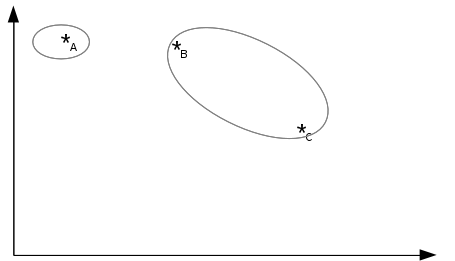
\includegraphics[scale=0.9]{kmeansInitCenters.png}
	\caption{Przykładowy podział początkowy obiektów grupowanych za pomocą algorytmu k-średnich. Punkt A leży bliżej punktu B niż punkt C, ale przy przedstawionym podziale początkowym środek grupy zawierającej punkty B i C będzie bliżej punktu B niż środek grupy zawierającej punkt A. Z tego powodu punkt B nie znajdzie się w grupie z najbardziej podobnym do niego punktem A.}
	\label{fig:kmeansInitCenters}
\end{figure}
	
Warto jeszcze wspomnieć, że algorytm ten jest za to prosty w implementacji i ma małą złożoność obliczeniową: O(n), gdzie n – jest liczbą obiektów wejściowych.

\myparagraph{Algorytm błędu kwadratowego}

Ten algorytm działa na podobnej zasadzie co powyższy, można go opisać następującymi krokami:

\begin{itemize}
	\item Wybierz początkowe wartości centrów grup. Liczba grup jest daną wejściową algorytmu.
	\item Przypisz każdy obiekt do jego najbliższego centrum. Oblicz nowe wartości centrów. Powtarzaj ten krok, dopóki nie zostanie spełniony warunek zakończenia – np. żaden obiekt nie zmienia grupy, żadna odległość obiektu od środka grupy nie przekracza zadanej wartości.
	\item Można podzielić lub połączyć pewne grupy, bazując na jakichś informacjach heurystycznych (na znajomości grupowanych danych), następnie można dodatkowo powtórzyć krok drugi.
\end{itemize}

\subsection{Grupowanie oparte na grafach}

W dosyć długiej historii algorytmów grupowania powstało kilka takich, które korzystają z teorii grafów. Jednym z nich – chyba najpopularniejszym w tej kategorii – jest algorytm tworzący dla danych wejściowych minimalne drzewo rozpinające. Wagi krawędzi w takim drzewie są odpowiednio wyznaczane na podstawie odległości dwóch obiektów od siebie, przy pomocy wybranej wcześniej miary odległości. Krawędzie z największymi wagami są usuwane, co prowadzi do powstania rozłącznych pod-grafów – podziałów wynikowych. Kryterium zakończenia może stanowić liczba uzyskanych podziałów albo średnia waga krawędzi w zbiorze krawędzi nieusuniętych.

Algorytm ten ma jedną dosyć poważną wadę. Jego wyniki są podobne do algorytmu grupowania hierarchicznego z wiązaniem pojedynczym – może wystąpić efekt łańcuchowy, czyli podział, w którym obiekty są od siebie bardzo różne, ale istnieje wśród nich jeden podobny, zapewniający przynależność do zbioru.

Używanie tego podejścia w grupowaniu jest związane z podejściem hierarchicznym. Oprócz analogii pomiędzy opisanym wyżej algorytmem, a wykorzystaniem wiązania pojedynczego istnieje jeszcze kilka podobieństw. Grupy powstałem poprzez użycie wiązania pełnego są takie same jak maksymalne, pełne pod-grafy minimalnego drzewa rozpinającego i są związane z kolorowanie wierzchołków grafu. Bibliografia jain 5.2.2

Aby otrzymać wyniki nie opisujące hierarchii podziałów można utworzyć graf Delaunay'a, \todo{Jain 5.2.2} który powstaje poprzez połączenie wszystkich par punktów, która są sąsiadami w rozumieniu kryterium Voronoi'a. Taki graf zawiera wszystkie informacje dotyczące sąsiedztwa zawarte w  algorytmie wykorzystującym minimalne drzewo rozpinające, oraz zawarte w grafie relatywnego sąsiedztwa.

\subsection{Inne rodzaje grupowania}

stnieją również inne sposoby wykonywania grupowania. Można je podzielić na takie jak grupowanie z wykorzystaniem kontekstu obiektu, z użyciem sieci neuronowych, ewolucyjne oraz na algorytmy stosujące pewne operacje w celu odnalezienia wzorców obiektów.

\myparagraph{Grupowanie kontekstowe}

Algorytm grupowania kontekstowego, zwany jest też grupowaniem najbliższego sąsiedztwa. Procedury grupowania, gdzie zastosowano takie podejście, rozpoczynają działanie od wielu jednoelementowych zbiorów obiektów. Obiekty łączy się w grupy, tworzone na podstawie łączenia ze sobą obiektów, które stanowią swoje bliskie sąsiedztwo (według ustalonego na początku kryterium). Sąsiedztwo to może być określane miarą liczby wspólnych sąsiadów, albo jedną z typowych miar odległości. Algorytm kończy się, gdy nie ma już wolnych obiektów lub gdy wolne obiekty nie dają się zakwalifikować do jednej z istniejących grup (są wtedy traktowane jako zakłócenia).

\myparagraph{Grupowanie rozmyte}

Typowe podejście do grupowania produkuje podziały, w których każdy obiekt należy do co najwyżej jednej grupy – jest to grupowanie dokładne, grupy są zawsze rozłączne. W podejściu alternatywnym pojęcie przynależności jest rozszerzane – poprzez użycie funkcji członkostwa próbuje się powiązać obiekt z każdą grupą, często opisując taką relację pewną wagą. Rezultatem wykonania takiego algorytmu jest pewien zbiór informacji o przynależności obiektów do grup, a nie jednoznaczny podział. Można opisać taki algorytm (z wysokiego poziomu abstrakcji) za pomocą następujących kroków:

\begin{itemize}
	\item Wybierz początkowy podział rozmyty N obiektów i K grup, tworząc macierz przynależności o wymiarach \[N\times K\] dalej oznaczaną symbolem U. Element $u_{i,j}$ tej macierzy reprezentuje stopień przynależności obiektu $x_{i}$ do grupy $c_{j}$. Zwykle \[u_{i,j} \in <0, 1> \]
	\item Wykorzystując U obliczyć wartość funkcji stanowiącej kryterium przydziału rozmytego, np. błąd średni kwadratowy. Możliwą rozmytą funkcją kryterium jest:
	\[E^2(X, U) = \sum_{i=1}^{N}\sum_{k=i}^{K}u_{i,j}||x_{i}-c_{k}||^2 \], gdzie \[ c_{k} = \sum_{i=1}^{N}u_{i,k}x_{i} \] jest k-tym rozmytym centrum grupy. Następnie przydziel obiekty do grupy tak, żeby zoptymalizować wartość funkcji kryterium i uaktualnij macierz U.
	\item Powtarzaj powyższy krok aż wszystkie wpisy w macierzy U nie będą się (znacznie) zmieniać.
\end{itemize}

\begin{figure}[H]
	\centering
	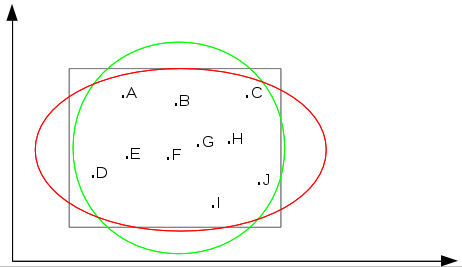
\includegraphics[scale=0.9]{rozmytewyniki.png}
	\caption{Wyniki grupowania rozmytego. Wszystkie grupy zostały przydzielone do każdej grupy - czerwonej, zielonej i szarej}
	\label{fig:rozmytewyniki}
\end{figure}

W grupowaniu rozmytym każda grupa to zbiór wszystkich obiektów. Przykładowe wyniki takiego grupowania są przedstawione na rysunku \ref{fig:rozmytewyniki}. Wchodząc głębiej w szczegóły takich wyników, można również założyć przykładowe wartości przynależności do każdej grupy:

\begin{table}[H]
	\centering
	\begin{tabular}{c|c|c|c|c|c|c|c|c|c|c}
		Grupa: & A & B & C & D & E & F & G & H & I & J \\ \hline
		czerwona & 50\% & 31\% & 74\% & 18\% & 25\% & 36\% & 19\% & 15\% & 8\% & 9\% \\ \hline
		zielona & 12\% & 11\% & 23\% & 14\% & 35\% & 17\% & 53\% & 58\% & 21\% & 22\% \\ \hline
		szara & 38\% & 58\% & 3\% & 68\% & 40\% & 47\% & 28\% & 27\% & 71\% & 69\%
	\end{tabular}
	\caption{Przykładowe wartości przynależności obiektów do grup w grupowaniu rozmytym.}
	\label{tab:rozmytewyniki}
\end{table}

Na podstawie danych jak w tabelce \ref{tab:rozmytewyniki} można uzyskać informacje o korelacji obiektów, albo wykonać szybkie grupowanie dokładne – przypisując obiekty do tych grup, z którymi mają najwyższą wartość przynależności.

\myparagraph{Grupowanie z użyciem sieci neuronowych}

Sztuczne sieci neuronowe (dalej nazywane skrótem SN) powstał w oparciu o biologiczne sieci neuronowe. SN znajdują szerokie zastosowania zarówno w zagadnieniach grupowania jak i w klasyfikacji. Kilka cech takich struktur jest szczególnie istotnych dla algorytmów grupowania:

\begin{itemize}
	\item SN operują na wektorach numerycznych, dlatego wymagają reprezentowania grupowanych obiektów za pomocą zbioru cech, z których każda jest przeliczalna.
	\item Struktura SN naturalnie narzuca / umożliwia realizowanie algorytmu grupowania w sposób równoległy / rozproszony.
	\item SN mają zdolność do uczenia się – potrafią zmieniać wagi połączeń pomiędzy neuronami w swojej strukturze. Prowadzi to do tego, że SN mogą nadawać dodatkowe wagi poszczególnym cechom, lub nawet całkowicie wykluczyć niektóre z nich z grupowania.
\end{itemize}

Do grupowania obiektów wejściowych często wykorzystywane są konkurujące SN (zwane też zwycięzca-bierze-wszystko, ang: winner-takes-all). W uczeniu konkurującym, obiekty podobne są grupowane przez całą sieć, a reprezentowane przez jeden neuron. Takie grupowanie wykonywane jest automatycznie na podstawie korelacji danych. \todo{Bibliografia, albo z jain albo z tego drugiego}

Dobrze znanymi przykładami SN wykorzystywanymi w grupowaniu jest sieć z kwantyzacją wektora uczącego (LVQ, ang: learning vector quantization), oraz samo-organizująca się mapa (SOM, ang: self-organizing map) jak również adaptacyjne modele teorii rezonansowej. Wagi pomiędzy węzłami wejściowymi i wyjściowymi są zmieniane iteracyjnie ( w ramach procesu uczenia się) dopóki warunek zakończenia algorytmu nie będzie spełniony. Istnienie takiej metody uczenia się zostało stwierdzone w biologicznych sieciach neuronowych.

SN typu SOM jako rezultat zwracają dwu-wymiarową mapę wielowymiarowego zbioru danych. Takie sieci z dobrymi wynikami używane do kwantyzacji wektorów oraz w algorytmach rozpoznawania mowy. Jednak ten typ SN generuje wyniki mogące nie być optymalnym podziałem na grupy – mają tendencję do zatrzymywania się w lokalnych optimach. Duży wpływ odgrywają tutaj parametry początkowe ustawiane jako wagi połączeń neuronów w sieci.

\myparagraph{Grupowanie ewolucyjne}

Jeszcze innym rodzajem jest grupowanie ewolucyjne, algorytmy tego typu powstały w oparciu o teorię ewolucji Darwina. Jeden podział nazywany jest chromosomem, zbiór podziałów jest populacją. Stosując operacje selekcji, mutacji i rekombinacji buduje się nowe zestawy podziałów. Na wejściu transformacji złożonej z kilku podstawowych operacji może być kilka podziałów, lub tylko jeden,  rezultatem zastosowanie transformacji również może być jeden lub kilka podziałów. Po pewnej liczbie iteracji algorytm powinien przynieść wyniki w postaci podziałów o stosunkowo wysokim współczynniku zdrowia (prawdopodobieństwa przeżycia). Przykładowe kroki takiego algorytmu można opisać w następujący sposób: 

\begin{itemize}
	\item Wybierz losową populację podziałów. Każdy podział odwzorowuje poprawny k-podział danych. Dla każdego podziału oblicz wartość współczynnika opisującego jego zdrowie i powiąż jego wartość z danym podziałem. Zwykle stosuje się współczynnik będący odwrotnością błędu kwadratowego. Podziały z mniejszym błędem mają większą wartość współczynnika zdrowia i tym samym większą szansę na przeżycie.
	\item Zastosuj operacje ewolucyjne selekcji, krzyżowania i mutacji do wygenerowania następnej populacji podziałów. Oblicz wartości współczynników zdrowia dla całej populacji. 
	\item Powtarzaj krok drugi dopóki nie będzie spełniony warunek zakończenia algorytmu (odpowiednio wysokie współczynniki przeżycie, bardzo podobne podziały w całej populacji).
\end{itemize}

Najbardziej znanymi technikami ewolucyjnymi są algorytmy genetyczne (zwane dalej GA, ang: genetic algorithms), strategie ewolucyjne (zwane dalej ES, ang: evolutionary strategies), oraz programowanie ewolucyjne (zwane dalej EP, ang: evolutionary programming). Z tych trzech metod w grupowaniu najczęściej używane jest GA. Punkty w przestrzeni poszukiwań (podziały) są reprezentowane jako łańcuchy binarne, stosowana jest operacja selekcji, rekombinacji (lekko zmodyfikowana – parę chromosomów łączy się dzieląc je na połowy i łącząc na krzyż) w celu przeszukania jak największej części przestrzeni podziałów. W celu upewnienia się, że cała przestrzeń została przejrzana, stosuje się również operację mutacji. ES i EP różnią się od GA stosowanymi operatorami i reprezentacją podziałów; w EP w ogóle nie jest stosowana operacja rekombinacji, w ES jest ona niezmodyfikowana – po prostu zamienia się losowo wybrane geny dwóch chromosomów. 

GA pozwala na wykonanie grupowania z globalnym poszukiwaniem rozwiązania – większość metod grupowania polega na poszukiwaniu lokalnym – takie poszukiwanie jest popularne ponieważ pozwala na zmniejszenie liczby bardzo kosztownych porównań wielowymiarowych wektorów cech. Produkcja podziałów w GA może znaleźć rozwiązania zupełnie inne od tych w poprzedniej operacji, natomiast w przeważającej większości przedstawionych w tym rozdziale algorytmów grupowania w kolejnych iteracjach mogą one tylko trochę zmienić podział znaleziony w poprzedniej iteracji. 

\myparagraph{Grupowanie oparte na wyszukiwaniu}

Techniki wyszukiwania stosowane w celu wyznaczenia optymalnej wartości funkcji kryterium są podzielone na deterministyczne i stochastyczne. Te pierwsze gwarantują otrzymanie wartości optymalnej poprzez wykonanie olbrzymiej liczby operacji. Z drugiej strony wyszukiwanie stochastyczne zapewnia rozwiązanie tylko bliskie optymalnemu, ale osiągane jest ono w rozsądnym czasie, a wartość funkcji kryterium asymptotycznie dąży do optimum. Pośród technik grupowania opisanych w tym rozdziale tylko te stosujące algorytmy ewolucyjne są stochastyczne, pozostałe można nazwać deterministycznymi. Inne znane metody deterministyczne to:

\begin{itemize}
	\item podziel-i-połącz (ang: branch-and-bound) – gwarantuje odnalezienie globalnego optimum, cechuje się bardzo wysokimi kosztami obliczeniowymi,
	\item deterministyczne wyżarzanie (ang: deterministic annealing) – przestrzeń błędu osiąga ciągłość i dąży do optymalnej, jednak ta metoda nie gwarantuje wykrycia globalnego optimum.
\end{itemize}

Typowo metodom deterministycznym można nadać kategorię metodologii zachłannych oraz zstępujących. Podejście stochastyczne zezwala na istnienie w przestrzeni rozwiązań odchyleń poza lokalnym optimum z niezerowym prawdopodobieństwem. Metody stochastyczne można podzielić na sekwencyjne lub równoległe, przy czym algorytmy ewolucyjne są zaliczane do kategorii równoległych. Do tej drugiej kategorii można zaliczyć stochastyczną metodę zwaną symulowanym wyżarzaniem (zwany dalej SA, ang. \textit{Simulated annealing}). Polega ona na dopuszczaniu, z pewnym prawdopodobieństwem, w kolejnej iteracji podziałów, które mają gorszą wartość funkcji kryterium. Prawdopodobieństwo akceptacji takiego podziału jest wyznaczone poprzez krytyczny parametr zwany temperaturą. Przykładowe kroki takiego algorytmu można opisać w następujący sposób:

\begin{itemize}
	\item Losowo wybierz początkowy podział $P_{0}$ oraz oblicz wartość błędu kwadratowego $E_{P0}$ dla tego podziału. Wybierz wartości parametrów sterujących, temperatury początkowej $T_{0}$ oraz temperatury końcowej (finalnej) $T_{f}$.
	\item Wybierz sąsiada $P_{0}$ oznacz go jako $P_{1}$ i oblicz dla niego wartość błędu kwadratowego $E_{P1}$ . Jeżeli $E_{P0}$ jest mniejsze od $E_{P1}$, to przypisz $P_{1}$ do $P_{0}$ z pewnym prawdopodobieństwem, zależnym od temperatury. W przeciwnym wypadku przypisz  $P_{1}$ do  $P_{0}$ . Powtarzaj ten krok ustaloną liczbę razy.
	\item Zmniejsz wartość $T_{0}$ stosując pewną ustaloną wartość $c: T_{0} = cT_{0}$. Jeżeli $T_{0}$ jest większe od $T_{f}$ , to idź do poprzedniego kroku. W przeciwnym wypadku zakończ algorytm.
\end{itemize}

Algorytm SA może być bardzo wolny w odnajdywaniu globalnego optimum, gdyż wymaga to od niego bardzo nikłego zmniejszania temperatury i powtarzania wyszukiwania z iteracji na iterację.

\myparagraph{Wyszukiwanie wzorców i algorytmy dekompozycji}

Założeniem leżącym u podstaw wyszukiwania wzorców jest to, że wszystkie obiekty w grupowanym zbiorze danych pochodzą od jednego z kilku obiektów wzorowych. Celem takiego algorytmu jest odnalezienie cech takiego obiektu oraz (czasem) liczby takich obiektów wzorowych. Większość prac w tej dziedzinie zakłada, że obiekty składające się na zbiór danych są składnikami nieokreślonej liczby dystrybuant Gaussa. Tradycyjne podejście do wykonania takiego algorytmu polega na tym, że iteracyjnie dopasowuje się parametry rozkładu Gaussa, oraz liczbę tych rozkładów (liczbę grup) tak, żeby uzyskać maksymalne prawdopodobieństwa wystąpienia wektorów opisujących obiekty w grupowanym zestawie danych.

Jednym z algorytmów realizujących takie podejście jest algorytm Maksymalizacji Wartości Oczekiwanej (ang. \textit{Expectation Maximization}). Generalnie stosuje się go do wyliczenia brakujących danych (np. podczas rekonstrukcji obrazków). Dla celów grupowania zakłada się, że parametry funkcji gęstości są nieznane, tak samo jak parametry mieszające – są one określane na podstawie obiektów. Procedura rozpoczyna się od przedstawienia początkowego wektora (wektorów) parametrów i na podstawie podobieństwa gęstości mieszaniny danych, które produkowane są poprzez zastosowanie tego wektora, ocenia się go przyrównując te dane do oryginalnego zbioru danych. Obiektom powstałym w sposób losowy nadaje się oceny (wagi) i tak zmodyfikowanych obiektów używa się do aktualizacji oszacowań parametrów. W kontekście grupowania oceny przyznane obiektom losowym (na podstawie ich podobieństwa do oryginalnych) mogą służyć do określenia, czy dany obiekt ze zbioru oryginalnego należy do grupy opisywanej przez dany wektor parametrów.

Zostały również opracowane bezparametrowe metody grupowania z wykorzystaniem funkcji gęstości. Wzorowana na oknie Parzena – metodzie do bezparametrowego oszacowania gęstości – procedura grupowania poszukuje kontenerów z dużą liczbą elementów w wielowymiarowych histogramach wejściowego zbioru obiektów. Jeszcze inne algorytmy tego typu wykorzystują podejście hierarchiczne lub partycjonujące, gdzie funkcją odległości jest bezparametrowe oszacowanie funkcji odległości. \todo{Doprowadzić to do takiego stanu, żeby było o wiele bardziej zrozumiałe. Odniesienia do bibliografii – jain 5.3.}

\myparagraph{Podsumowanie}

Warto zaznaczyć, że można również stosować algorytmy hybrydowe. Polega to na zastosowaniu do jednego zbioru danych różnych typów algorytmów, i ustaleniu wyniku na przykład poprzez głosowanie – nadając poszczególnym wynikom różne wagi, ustalone na drodze eksperymentów. Każdy z użytych algorytmów może na wejściu otrzymać taki sam opis obiektów, albo tylko częściowy – pozwalający na jak najbardziej efektywne wykorzystanie danego algorytmu. Podział danych wejściowym między różne algorytmy może się opierać na logice związanej z grupowanymi obiektami. Można na przykład wykonać grupowanie na wektorach cech obliczonych na podstawie bibliografii i liczby odwołań do niej, wyznaczonej dla każdego dokumentu znajdującego się w zadanym zbiorze. Dołączyć do tego grupowanie wykonane na podstawie abstraktów dokumentów i grupowanie przeprowadzone na podstawie całej treści. Tak powstałe 3 wyniki grupowania można opisać za pomocą wektora cech informującego o podobieństwie dokumentów w każdym z tych 3 rezultatów i przeprowadzić na tym kolejne grupowanie.
Rozwiązanie takie może dać bardzo dokładne wyniki, odwzorowując faktyczne podobieństwo tematyczne badanych dokumentów, ale jednocześnie byłoby bardzo kosztowne czasowo. \todo{Wstawić odwołanie do rozdziału lub bibliografii, gdzie będą przeprowadzone podobne eksperymenty, uzasadnienie dlaczego to będzie kosztowne.}

\subsection{Sposoby reprezentacji grup}

Rezultat działania programu grupującego dane, powinien pozwolić wnioskować o 
 \begin{itemize}
 	\item rozłączności danych,
 	\item gęstości danych,
 	\item jakości grupowania (średni błąd, porównanie z innymi wynikami, wizualizacja).
 \end{itemize}
 Na przykład przy niskiej jakości wynikowego grupowania użytkownik mógłby ponowić procedurę zadając inne parametry wejściowe. 
 \\
 Dodatkowo taki program powinien pozwolić zapisać podział na grupy w taki sposób, żeby nie zajmował dużo pamięci i był łatwy do interpretacji przez inne programy. Pomimo istotnej wagi zagadnienia reprezentacji wyników grupowania, temat ten nie był \todo{Jain 5.6} przedmiotem wnikliwych badań. Spośród istniejących rozważań warto rozpatrzyć następujące:

\begin{itemize}
	\item Reprezentowanie grupy punktów poprzez środek tej grupy (Rysunek \ref{fig:gruparepsrod}) lub przez zbiór najbardziej odległych od siebie punktów (Rysunek \ref{fig:gruparepodlegle}).
	\item Reprezentacja grup poprzez węzły w drzewie klasyfikacji (Rysunek \ref{fig:klasdrzewo}).
	\item Reprezentacja poprzez ciąg koniunkcji wyrażeń logicznych opisujących każdą grupę. Na przykład opisując podział z rysunku \ref{fig:klasdrzewo} uzyskalibyśmy następujący ciąg:
	\[ niebieska:[X<4,5]; czerwona:[X>4,5]\vee[Y>1,5]; żółta:[X>4,5]\vee[Y<1,5] \]
\end{itemize}

\begin{figure}[H]
	\centering
	\begin{subfigure}{.5\textwidth}
		\centering
		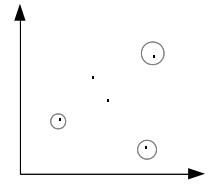
\includegraphics[scale=0.75]{gruparepodlegle.png}
		\caption{Okręgiem zostały zakreślone najbardziej odległe od siebie punkty - stanowiące reprezentację przedstawionej grupy.}
		\label{fig:gruparepodlegle}
	\end{subfigure}%
	\begin{subfigure}{.5\textwidth}
		\centering
		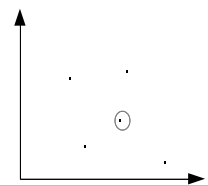
\includegraphics[scale=0.75]{gruparepsrod.png}
		\caption{Okręgiem został zaznaczony punkt będący środkiem grupy.}
		\label{fig:gruparepsrod}
	\end{subfigure}
\end{figure}

\begin{figure}[H]
	\centering
	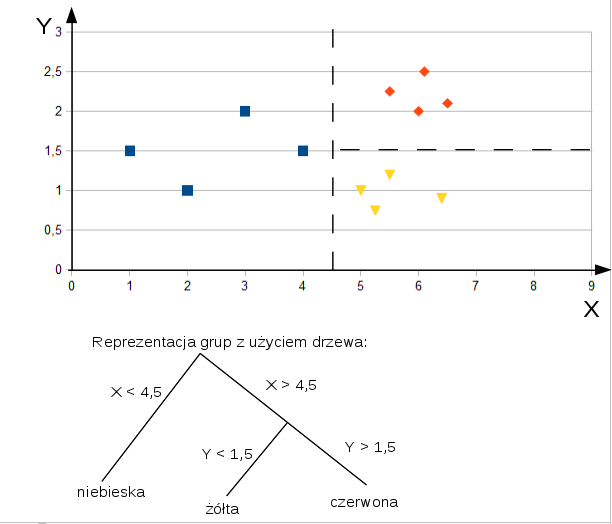
\includegraphics[scale=0.75]{klasdrzewo.png}
	\caption{Przykładowy podział na grupy i drzewo klasyfikacji}
	\label{fig:klasdrzewo}
\end{figure}

Każdy element z powyższego wyrażenia stanowi opis poszczególnej gałęzi z drzewa zaprezentowanego na rysunku \ref{fig:klasdrzewo}. Ważnym ograniczeniem dla tego sposobu reprezentacji grup jest fakt, że da się w ten sposób opisać jedynie grupy izotropowe lub prostokątne w swojej przestrzeni cech.

Najpopularniejszym sposobem reprezentacji grup jest użycie środków. Dobrze się to sprawdza dla grup zwartych oraz dla grup jednorodnych (izotropowych). Jednak dla grup rozciągniętych lub nie-izotropowych taka reprezentacja zawodzi. Praktyka pokazuje, że lepiej użyć kolekcji punktów granicznych (najbardziej odległych). Oczywiście liczba punktów wykorzystanych do reprezentacji grupy rośnie wraz ze skomplikowaniem kształtu reprezentowanej grupy.

Reprezentacja danych jest istotnym zagadnieniem związanym z użyteczności algorytmów grupowania, ponieważ:

\begin{itemize}
	\item Może zapewnić prosty i intuicyjny opis grup, łatwy do zrozumienia przez ludzi. Niektóre sposoby grupowania zapewniają wyprodukowanie takiej reprezentacji bez żadnego dodatkowego kroku.
	\item Może pomóc w przeprowadzeniu stratnej kompresji danych, co zostało zaprezentowane na rysunku \ref{fig:kompresjagrup}. Otrzymane za pomocą grupowania np. algorytmem k-średnich grupy mogą być reprezentowane przez ich środki.
	\item {Może przyspieszyć proces podejmowania decyzji i wyszukiwania danych. Po wykonaniu grupowania wyszukiwanie można przeprowadzać na uzyskanych środkach grup, i dopiero otrzymując potencjalnie interesujące grupy, można przeglądać ich zawartość.}
\end{itemize}

\begin{figure}
	\centering
	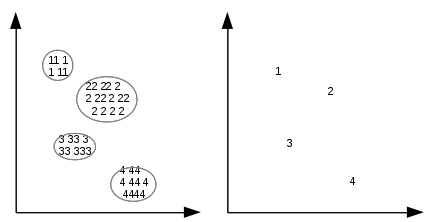
\includegraphics[]{kompresjagrup.png}
	\caption{Lewy wykres przedstawia zgrupowane dane przed kompresją, prawy po kompresji.}
	\label{fig:kompresjagrup}
\end{figure}

\newpage
\section{Grupowanie dokumentów}

Dokumenty różnią się trochę od innych rodzajów obiektów, szczególnie z punktu widzenia grupowania \todo{4}. Bez wątpienia można powiedzieć, że dwa dokumenty zawierające prawie identyczną sekwencję słów, powinny się znaleźć w jednej grupie. Jednak proces porównywania dokumentów jest bardzo kosztowny. Każde słowo w dokumencie jest kolejnym wymiarem – kolejną cechą w wektorze cech. Dodatkowo konieczna jest obróbka wstępna takich danych. Wyłuskanie treści z plików o różnych formatach i odpowiednie jej zachowanie. 

\subsection{Obróbka wstępna}

Aby przygotować dokumenty do przetwarzania przez algorytm grupowania danych, należy wykonać kilka niezbędnych kroków.

Pierwszym jest sprowadzenie dokumentu do surowej formy tekstowej [2]. Wymaga to użycia różnych narzędzi odczytujących rozmaite formaty plików, takie jak pdf, odt, doc czy docx. Następnie dokument może być przefiltrowany – pozbawiony dat, numerów, znaków nieistotnych z punktu widzenia grupowania. Kolejnym krokiem jest sprowadzenie słów w dokumencie do unikalnych form podstawowych, dzięki czemu porównanie dokumentu będzie o wiele łatwiejsze: na przykład odmiany słowa grupowanie (takie jak grupowania, grupowaniem, itp) będą reprezentowane takim samym tematem (np. grupow). Uzyskany zbiór można ponownie przefiltrować, na przykład na podstawie jakiegoś słownika, zawierającego terminy, które w danym języku nie są istotne dla znaczeniu dokumentu.

Po powyższych operacjach można zliczyć liczby wystąpień poszczególnych unikalnych form (w praktyce można to robić jednocześnie z ujednolicaniem form słów – wpływa to na zwiększenie efektywności) i na tej podstawie utworzyć wektor słów dla dokumentu. Gdy już każdy dokument w przetwarzanym zbiorze ma swój wektor słów, to łączy się je w wektor opisujący cały zbiór – zawierający liczbę wystąpień unikalnych form słów w całym zbiorze. Dodatkowo na podstawie takich wektorów można zbudować histogramy dokumentów (lokalne – dla jednego dokumentu i globalne – dla całego zbioru). Na ich podstawie można przeprowadzić dodatkową filtrację, obcinając oba końce histogramu – jako słowa zbyt rzadko i zbyt często występujące, aby mogły stanowić o odpowiednim podziale zbioru dokumentów na mniejsze zbiory. Należy jednocześnie pamiętać, że taka operacja może zaszkodzić podziałowi. Być może w badanym zbiorze początkowym istnieje po prostu nadreprezentacja pewnej kategorii dokumentów, lub bardzo mała reprezentacja innej kategorii. Ucięcie końców histogramu może uniemożliwić identyfikację takich zjawisk.

\subsection{Wektor cech}

Właściwy wektor cech do porównywania dokumentów buduje się na podstawie indeksu tf*idf (ang. \textit{Term frequency – inverse document frequency}). Indeks ten, wyraża się następującym wzorem \todo{1,3}:

\[ tf*idf(t, d, D) = tf(t, d)\times idf(t, D) \]

Gdzie tf dla i-tego słowa w zbiorze, w n-tym dokumencie to (x oznacza liczność danego słowa):

\[ tf(t_{i}, d) = x_{n,i} / \sum_{k=1}^{len(d_{n})}x_{n,k} \]

Dla współczynnika tf zachodzi zależność: \[ tf == 1 \leftrightarrow x_{n,i} == \sum_{k=1}^{len(d_{n})}x_{n,k} \]

Oznacza to, że pierwsza część współczynnika $tf \times idf$ może być równa 1 tylko wtedy, jeżeli badane słowo jest jedynym słowem występującym w danym dokumencie. W każdym innym wypadku ta część będzie mniejsza niż 1. 

Natomiast $idf$ to dla i-tego słowa w n-tym dokumencie to: 

\[ idf(t, D) = \log(\frac{|D|}{|d \in D: t_{i} \in d|})  \]

Jak widać, współczynnik $idf$ nie zależy od n-tego dokumentu, natomiast ułamek znajdujący się w logarytmie nigdy nie będzie przyjmować wartości mniejszych od 1:
\begin{itemize}
	\item $D$ to liczba wszystkich rozpatrywanych dokumentów
	\item $|d \in D: t_{i} \in d|$ to liczba dokumentów w których występuje rozpatrywane słowo - z racji tego, że pod uwagę brane są tylko słowa, które znajdują się w zbiorze dokumentów, nie ma obawy, wartość ta będzie zero - i nie zajdzie dzielenie przez zero. 
\end{itemize}
Maksymalna wartość mianownika to $D$, co oznacza, że słowo występuje w każdym dokumencie w analizowanym zbiorze. Argument logarytmu $\log(\frac{|D|}{|d \in D: t_{i} \in d|})$ sprowadza się wtedy do wartości $1$, co oznacza, że cały współczynnik $tf \times idf$ będzie równy 0.

Dodatkowym zabiegiem przy obliczaniu takiego wektora jest uwzględnienie semantyki słów. Przy pomocy słownika wyrazów bliskoznacznych automat jest w stanie zastąpić różne słowa o podobnym znaczeniu jednym i tym samym, modyfikując odpowiednio wagi w wektorze cech – poprzez dodanie nowych wartości podczas obliczania tf i idf, ewentualnie z wagami, żeby uwzględnić, że dane słowo może mieć trochę inne znaczenie \todo{2}.

Innym \todo{Podać przykład, albo odniesienie do bibliogrrafi [jain] albo coś o dokumentach } często stosowanym zabiegiem jest wykorzystanie słowników terminologii, do pozostawienia w wektorze cech tylko żądanych słów, lub usunięcia niepożądanych. W przypadku zbioru wejściowego w postaci tekstów z dziedziny medycyny, traktujących o różnych nowotworach, pomogłoby to usunąć część treści, które nie dotyczy bezpośrednio nowotworów i umożliwiłoby grupowanie wyłącznie ze względu na rodzaje nowotworów.

\subsection{Porównanie dokumentów}

Zwykle wykonuje się porównanie wektorów cech dokumentów (obliczenie odległości pomiędzy nimi) \todo{[4]}. Jednak istnieją alternatywne metody. 

Jedną z możliwości jest zbudowanie wektora cech tylko dla części dokumentu (na przykład dla abstraktu). Spowoduje to zapewne utratę części istotnych informacji, ale znacznie przyspieszy proces grupowania. Pozwoli to użytkownikowi uzyskać mniej dokładne wyniki, ale w krótszym czasie, co może stanowić dużą zaletę rozwiązania. 

Dokumenty takie jak artykuły naukowe często są wzbogacone o słowa kluczowe, dodane przez autorów artykułów, co może stanowić jeszcze lepsze niż abstrakt i jednocześnie wystarczające źródło informacji o tematyce dokumentu. Jednak wykorzystanie cech dokumentów, które są specyficzne dla danego typu dokumentu, wykluczyłoby uniwersalność rozwiązania.

Drugą metodą jest porównywanie dokumentów za pomocą ich bibliografii. Każdy artykuł zawiera odniesienia do innych artykułów, przy czym czasem są to odniesienia pojedyncze, a czasem jedno odniesienie adresowane jest do kilku innych artykułów jednocześnie. Zliczając takie odniesienia w tekście dokumentu, oraz nadając im odpowiednie wagi, zależne od:

\begin{itemize}
	\item częstości odniesień do danej pozycji z bibliografii
	\item liczebności pozycji w ramach jednego odniesienia, w którym występuje interesująca nas pozycja
	\item miejsce w dokumencie, w którym wystąpiło odniesienie (analiza wyników takiego grupowania mogłaby wykazać, że na przykład ważniejsze są odniesienia ze środkowych rozdziałów, od tych z końcowych – tu jednak pojawia się problem identyfikacji różnych obszarów w dokumencie).
\end{itemize}
Tak określone wagi można wykorzystać jako odległości pomiędzy dokumentami. Posiadając takie informacje można zbudować graf sąsiedztwa dokumentów, z wagami które opisywałyby stopień sąsiedztwa – im większy tym dokumenty są bliżej do siebie. 

W celu zgrupowania takich dokumentów na podstawie jakiejś zadanej kategorii, trzeba byłoby dla części tych dokumentów wprowadzić tagi – słowa kluczowe, lub treść abstraktu. Nadanie takich słownych znaczników tylko części dokumentów w grafie wystarczyłoby, ponieważ reszta oznaczeń propagowałaby się na inne dokumenty na podstawie podobieństwa. Zagadnieniem, które należałoby rozwiązać jest liczba dokumentów, które trzeba oznaczyć w grafie, żeby wyniki grupowania były dobre, oraz dobór takich dokumentów – czy lepiej brać dokumenty znajdujące się w wierzchołkach o wyższych stopniach, czy może lepiej te, które są w wierzchołkach o niskim stopniu.

\subsubsection{Algorytm k-średnich}

Algorytm k--średnich jest najczęściej wykorzystywanym algorytmem grupowania dokumentów \todo{Tutaj odwołanie do artykułu $itereative_icdm2$ - już w abstrakcie o tym wspominają}. Najczęściej wykorzystywany jest razem z funkcją określającą podobieństwo wektorów na podstawie podobieństwa cosinusowego. Dokładny opis działania takiego algorytmu można znaleźć w wielu źródłach \todo{Podać jakie źródła}. 

W podstawowej wersji algorytm ten posiada złożoność obliczeniową równą $O(n^{kd+1}log n)$ , gdzie:
\begin{itemize}
	\item n – liczba obiektów do zgrupowania,
	\item k – liczba grup oczekiwana na wyjściu algorytmu,
	\item d – liczba wymiarów wektorów opisujących zadane obiekty.
\end{itemize}
Każdy obiekt trzeba porównać ze wszystkimi środkami (w najgorszym wypadku), w każdej iteracji algorytmu. Na koniec każdej iteracji obliczane są nowe centra grup, które wektorami średnimi ze wszystkich wektorów w danej grupie. Dodatkowo samo porównanie dwóch wektorów to obliczenie ich podobieństwa, czyli w przypadku podobieństwa cosinusowego jest to $d^2$ operacji.

\todo{podobieństwo cosinusowe nie zależy od długości wektorów – dlatego najwydajniej jest obliczać je na podstawie wektorów znormalizowanych mk-cos-euclidean,
	podobieństwo cosinusowe nie spełnia nierówności trójkąta – źródło jak wyżej
	takie wektory można próbować sprowadzać do wektorów skwantowanych – testy z wartością kwantyzacji, dobieranie heurystycznie na podstawie mediany wartości wszystkich współrzędnych, albo na podstawie średniej wszystkich współrzędnych, albo na podstawie średniej / mediany współrzędnych dla każdego wektora osobno.}

\newpage
\section{Implementacja rozwiązania}
W celu zbadania skuteczności metod grupowania zaimplementowany został algorytm k-średnich, z kilkoma rodzajami wyboru początkowego:
\begin{itemize}
	\item Wybór losowy - funkcja prawdopodobieństwa o rozkładzie jednostajnym jest użyta aby przypisać każdy punkt do jednej z grup.
	\item Wybór sekwencyjny - punkty po kolei są dodawane do kolejnych grup. Przy 3 grupach i 8 punktach (załóżmy że są indeksowane od 0 do 7), punkty o indeksach 0, 3 i 6 będą w pierwszej grupie, punkty o indeksach 1, 4, 7 znajdą się w drugiej grupie, a do grupy trzeciej trafią punkty o indeksach 2 i 5.
	\item Wybór na podstawie minimalnego drzewa rozpinającego dla l-pierwszych punktów - ten sposób wybierania podziału początkowego jest opisany w podrozdziale \todo{dodać ten podrozdział}
\end{itemize}

Dodatkowo zostały zaimplementowane funkcje do obliczania odległości hamiltona, hamminga, euclidesa i cosionusowej - wybór funkcji podobieństwa może wpłynąć na wyniki grupowania. W dalszej części pracy przedstawione będzie porównanie wyników ze względu na użytą funkcję odległości.

\subsection{Wybór podziału początkowego na podstawie minimalnego drzewa rozpinającego}

Istnieją już wersje algorytmu k-means używające minimalnego drzewa rozpinającego, \todo{referencja do http://waset.org/publications/10006049/a-minimum-spanning-tree-based-method-for-initializing-the-k-means-clustering-algorithm} gdzie zaznaczono, że użycie takiego drzewa pozwala przyspieszyć i poprawić działanie algorytmu grupującego - na co wskazuje lepsza niż dla innych grupowań wartość indeksu grupowania asocjacyjnego. Jednak w przypadku danych tekstowych, których grupowanie jest przedmiotem tej pracy, użycie minimalnego drzewa rozpinającego może dać jeszcze większe przyspieszenie, a zbudowanie go będzie kosztować mniej, niż w przypadkach opisanych w artykule \todo{tym co wyżej}. 
Dane tekstowe charakteryzują się:
\begin{itemize}
	\item dużą liczbą wymiarów - każdy wymiar to unikalne słowo znajdujące się w jednym z dokumentów będącym częścią grupowanego zbioru;
	\item znaczącą liczbą wymiarów zerowych - w wielu korpusach dostępnych w internecie, spośród całej dziedziny słów dostępnej w korpusie, w dokumencie występuje średnio nie więcej niż 25\% wszystkich słów \todo{linki do korpusów i dokładna liczba}
\end{itemize}
Dzięki takiej charakterystyce, można użyć odległości hamminga dla wykonania podziału początkowego i tym samym przyspieszyć jego wygenerowanie. Każdorazowe obliczenie odległości hamminga jest szybsze niż obliczanie odległości euklidesowej.

\subsubsection{Opis wyboru podziału początkowego}

W tej wersji algorytmu podział początkowy wybierany na podstawie minimalnego drzewa rozpinającego oparty jest na algorytmie zachłannym i dopasowanym do zadanej na wejściu liczby wymiarów.

\begin{enumerate}
	\item Pierwszym krokiem jest obliczenie odległości hamminga pomiędzy wszystkimi wektorami cech, i przypisanie każdemu wektorowi nowej cechy - jego sumarycznej odległości od wszystkich pozostałych punktów. Jednocześnie wybierana jest najmniejsza odległość między dwoma punktami, jaka występuje w tym zbiorze danych i odległość ta jest ustawiana jako aktualny dystans maksymalny.
	\item Punkty są sortowane ze względu na swoją sumaryczną odległość od pozostałych - na początku ustawiane są punkty z najmniejszą wartością tego parametru.
	\item Ustaw aktualnie obsługiwaną grupę na pierwszą.
	\item Dla każdego punktu wykonywane są następujące kroki, dopóki każdy z punktów będzie miał przypisaną grupę:
	\begin{enumerate}
		\item \label{krok1} Wybierz punkt z początku listy - z najmniejszą sumaryczną odległością - i przypisz go do aktualnie obsługiwanej grupy, a następnie usuń go z tej listy.
		\item \label{krok2} Dla wszystkich punktów, z którymi ten punkt sąsiaduje, sprawdź z czy dzieląca go odległość jest mniejsza lub równa od aktualnego dystansu maksymalnego.
		\item Dla każdego punktu sąsiadującego który przeszedł to sprawdzenie, dodaj go do aktualnie obsługiwanej grupy i usuń z listy. Następnie dla każdego z nich powtórz krok \ref{krok2} i kolejne, aż do wyczerpania takich punktów.
		\item Jeżeli żaden punkt nie przeszedł sprawdzenia z kroku \ref{krok2}, zmień aktualną grupę na kolejną.
		\item Pod warunkiem, że wybrana grupa jeszcze nie była obsługiwana przy aktualnym dystansie minimalnym, przejdź do \ref{krok1}, w przeciwnym wypadku idź do kolejnego kroku.
		\item Zwiększ aktualny dystans minimalny o odległość minimalną i przejdź do kroku \ref{krok1}.
	\end{enumerate}
\end{enumerate}

\newpage
\section{Testy i wnioski}

Testy były wykonane na zbiorze artykułów naukowych dotyczących różnych dziedzin prawa. Każdy z nich posiada wyróżnione sekcje na abstrakt, słowa kluczowe, i kolejne rozdziały. Wszystkie są w języku angielskim. Zostały pobrane ze strony \todo{http://reference.findlaw.com/lawandeconomics/contents.html}.

\subsection{Obróbka danych tekstowych}

Zanim jakiekolwiek grupowanie czy wybór podziałów początkowych mogą mieć miejsce, artykuły w plikach pdf trzeba sprowadzić do postaci wektorów cech tfidf. 
Aby to osiągnąć potrzebne były następujące kroki:

\begin{enumerate}
	\item Pierwszym krokiem była konwersja każdego artykułu z formatu pdf, do formatu tekstowego. Użyto do tego jednej z liczny stron oferujących takie konwertery za darmo \todo{http://pdftotext.com/pl/}.
	\item Kolejnym krokiem było napisanie i wywołanie skryptu w języku Python, który posiada biblioteki do procesowania języka naturalnego\todo{python nlp}. Zanim jednak można było użyć bibliotek do obróbki tekstu, trzeba było ujednolicić format plików, oraz pozbyć się artefaktów pozostałych po konwersji z formatu pdf na tekstowe:
	\begin{enumerate}
		\item Usunięcie numerów stron, stopek oraz nagłówków (zawierających np. tytuł artykułu, autorów, itp.).
		\item Usunięcie znaków nie będących standardowymi dla zdań po angielsku (czyli różnych typów cudzysłowów, podłużnych myślników, itp.)
		\item Podział logiczny dokumentu na części typowe dla artykułów naukowych: abstrakt, słowa kluczowe, wstęp i kolejne rozdziały, bibliografia.
	\end{enumerate}
	\item Po zakończonej wstępnej obróbce, powstawały 4 dokumenty, na każdy artykuł, zawierające:
	\begin{itemize} \label{doc_types}
		\item tylko abstrakt artykułu;
		\item wstęp i pozostałe rozdziały - bez bibliografii;
		\item słowa kluczowe
		\item abstrakt, wstęp oraz wszystkie rozdziały, bez bibliografii.
	\end{itemize}
	\item każdy z wymienionych wynikowych zbiorów danych został poddany następującej obróbce: 
	\begin{enumerate}
		\item podział artykułu na zdania, przy użyciu \textit{nltk.tokenize},
		\item rozbicie zdań na słowa i oznaczenie tych słów częściami mowy i zdania przy użyciu modułu j.w.,
		\item sprowadzenie formy fleksyjne słów do postaci słownikowej, na podstawie przydzielonych im oznaczeń części mowy i zdania, przy użyciu lematyzera \textit{WordNet},
		\item usunięcie wyrazów pospolitych (ang. \textit{stopwords}) za pomocą słownika z modułu \textit{nltk.corpus.stopwords}
		\item przekształcenie formy słownikowej do rdzenia z wykorzystaniem modułu \textit{stemming.porter2}.
	\end{enumerate}
\end{enumerate}

Po zakończonym procesie nastąpił etap ręcznego sprawdzenia wynikowych dokumentów - w celu zweryfikowania jakości procesu. W sytuacji, gdy w zbiorze słów znajdowały się słowa nie sprowadzone do rdzenia (na przykład przez przylegający do nich zestaw cudzysłowów dolnych, przechylonych w lewo), implementowane były poprawki do skryptu (na przykład usuwające określone znaki z tekstu), mające na celu tą jakość poprawić. 

Ostatecznie otrzymano następujące zbiory słów:
\begin{itemize}
	\item Abstrakty - 1841 słów
	\item Rozdziały - 36907 słów
	\item Całość - 36938 słów
	\item Słowa kluczowe - 559 słów.
\end{itemize} 
Tak powstałe dokumenty można było przerobić na wektory cech dokumentów, używając wskaźnika \[tf \times idf \] do przekształcenia zbiorów słów na liczby.
Jednak zanim ten krok zostanie wykonany, należy zwrócić uwagę na to, że liczba unikalnych słów dla każdego z tych typów dokumentów ciągle jest duża, i na pewno znajdują się tam słowa, które można pominąć. 
Dla każdego słowa została policzona jego wariancja - biorąc pod uwagę liczność występowania słowa w całym zbiorze artykułów. Na podstawie wyliczonej wariancji stworzone zostały dodatkowe zbiory dokumentów do analizy:
\begin{itemize}
	\item Abstrakty, gdzie minimalna dopuszczalna wariancja to 1, liczba słów to
	\item Rozdziały, gdzie minimalna dopuszczalna wariancja to 1, liczba słów to
	\item Rozdziały, gdzie minimalna dopuszczalna wariancja to 5, liczba słów to
	\item Całość, gdzie minimalna dopuszczalna wariancja to 1, liczba słów to
	\item Całość, gdzie minimalna dopuszczalna wariancja to 10, liczba słów to
	\item Całość, gdzie minimalna dopuszczalna wariancja to 20, liczba słów to
	\item Całość, gdzie minimalna dopuszczalna wariancja to 40, liczba słów to
\end{itemize}

\subsection{Wyniki grupowania porównawczego}

Do grupowania porównawczego użyty został algorytm LDA \todo{opisać, napisać że trwał około 4-5h i dał RAND ~0,84}.

\subsection{Wyniki grupowania}

\begin{table}[H]
	\centering
	\begin{tabular}{c|c|c}
		(w sekundach) & $tf \times idf$ i generowanie słownika & $tf \times idf$ na podstawie słownika \\ \hline
		Abstrakty: & 0,47 & 0,03 \\ \hline
		Rozdziały & 13,82 & 3,81 \\ \hline
		Całość & 14,46 & 3,52 \\ \hline
	\end{tabular}
	\caption{Czasy obliczenia tfidf i wygenerowania słownika słów ignorowanych, oraz wykonania tfidf na postawie słownika.}
	\label{tab:tfidfczas}
\end{table}


\begin{table}[H]
	\centering
	\begin{tabular}{c|c|c}
		Indeks RAND & odległość Hamminga & odległość euklidesowa \\ \hline
		P.p. sekwencyjny: & 0,792857 & 0,792857 \\ \hline
		P.p. losowy: & 0,792857 & 0,802521  \\ \hline
		P.p. MST: & 0,339076 & 0,339076 \\hline
		P.p. sekwencyjny, Varx = 1: & 0,707563 & 0,686275 \\ \hline
		P.p. losowy, Varx = 1: & 0,714846 & 0,732073  \\ \hline
		P.p. MST, Varx = 1: & 0,714426 & 0,714426
		\end{tabular}
		\caption{Wyniki grupowania na podstawie abstraktów. P.p - podział początkowy; MST -na podstawie minimalnego drzewa rozpinającego. Słowa były odcinane przy wariancji równej 1.}
		\label{tab:abstraktywyniki}
\end{table}

\begin{table}[H]
	\centering
	\begin{tabular}{c|c|c}
		Indeks RAND & odległość Hamminga & odległość euklidesowa \\ \hline
		P.p. sekwencyjny: & 0,736835 & 0,763025 \\ \hline
		P.p. losowy: & 0,758683 & 0,671569 \\ \hline
		P.p. MST: & 0,675910 & 0,560224 \\ \hline
		P.p. sekwencyjny, Varx = 1: & 0,754342 & 0,652241 \\ \hline
		P.p. losowy, Varx = 1: & 0,743978 & 0,593557 \\ \hline
		P.p. MST, Varx = 1: & 0,795238 & 0,635154 \\ \hline
		P.p. sekwencyjny, Varx = 5: & 0,668768 & 0,643557 \\ \hline
		P.p. losowy, Varx = 5: & 0,139776 & 0,62535  \\ \hline
		P.p. MST, Varx = 5: & 0,709384 & 0,702241
	\end{tabular}
	\caption{Wyniki grupowania na podstawie rozdziałów. P.p - podział początkowy; MST -na podstawie minimalnego drzewa rozpinającego; VarX - odcięcie słów przy danej wariancji.}
	\label{tab:rozwyniki}
\end{table}

\begin{table}[H]
	\centering
	\begin{tabular}{c|c|c}
		Indeks RAND & odległość Hamminga & odległość euklidesowa \\ \hline
		P.p. sekwencyjny: & 0,736835 & 0,754622 \\ \hline
		P.p. losowy: & 0,758403 & 0,647619  \\ \hline
		P.p. MST: & 0,649020 & 0,649020 \\ \hline
		P.p. sekwencyjny, Varx = 1: & 0,776331 & 0,658543 \\ \hline
		P.p. losowy, Varx = 1: & 0,751541 & 0,602381  \\ \hline
		P.p. MST, Varx = 1: & 0,658263 & 0,658263 \\ \hline
		P.p. sekwencyjny, Varx = 10: & 0,637255 & 0,661905 \\ \hline
		P.p. losowy, Varx = 10: & 0,602941 & 0,540476  \\ \hline
		P.p. MST, Varx = 10: & 0,741176 & 0,741176 \\ \hline
		P.p. sekwencyjny, Varx = 20: & 0,601120 & 0,674650 \\ \hline
		P.p. losowy, Varx = 20: & 0,609384 & 0,523529  \\ \hline
		P.p. MST, Varx = 20: & 0,627871 & 0,627871 \\ \hline
		P.p. sekwencyjny, Varx = 40: & 0,511905 & 0,596359 \\ \hline
		P.p. losowy, Varx = 40: & 0,570028 & 0,551120  \\ \hline
		P.p. MST, Varx = 40: & 0,690756 & 0,690756
	\end{tabular}
	\caption{Wyniki grupowania na podstawie całości. P.p - podział początkowy; MST -na podstawie minimalnego drzewa rozpinającego; VarX - odcięcie słów przy danej wariancji.}
	\label{tab:calwyniki}
\end{table}

\begin{table}[H]
	\centering
	\begin{tabular}{c|c|c}
		Indeks RAND & odległość Hamminga & odległość euklidesowa \\ \hline
		P.p. sekwencyjny: & 0,744398 & 0793137, \\ \hline
		P.p. losowy: & 0,799440 & 0,800560  \\ \hline
		P.p. MST: & 0,200980 & 0,589776 
	\end{tabular}
	\caption{Wyniki grupowania na podstawie słów-kluczy. P.p - podział początkowy; MST -na podstawie minimalnego drzewa rozpinającego. Grupowanie było wykonane bez usuwania terminów, jako że słów kluczowych było od początku bardzo mało.}
	\label{tab:keywordswyniki}
\end{table}

We wszystkich tabelach \ref{tab:abstraktywyniki}, \ref{tab:rozwyniki}, \ref{tab:calwyniki} wartości zostały zaokrąglone do 6-tego miejsca po przecinku. Stąd niektóre z wartości wyglądają tak samo - na przykład w tabeli \ref{tab:calwyniki} grupowanie przy użyciu podziału opartym na minimalnym drzewie rozpinającym ma takie same wartości indeksu RAND, bez względu na rodzaj użytej funkcji odległości. Możliwe, że algorytm wpada w lokalne minimum i nie da lepszego wyniku \todo{dodać liczbę użytych iteracji do wyników, dodać czasy wykonania}. 

Wszystkie algorytmy odcinały słowa, o wariancji liczności mniejszej niż jeden, lub większej - jak podane w tabelkach. Widać, że zbyt duże odcięcie nie poprawia wyników grupowania\todo{Ciekawe, poprawić wariancje - do niższej, sprawdzić}.

\newpage
\section{notatki robocze}
W rozdziale 2 dodać teorię.
	6.02 spotkanie o 17
	1. Dodać bez wariancji
	1.1 Jak ocenić grupowanie, podobieństwo
	1.2 Rodział cały o ocenie grupowania
	2. Uzasadnić wybór funkcji odległości – opisać działaniu ich obu, odniesienie do bibliografii. Prezentacja testów ich wydajności ze względu na liczbę wymiarów, gęstość wektorów, rodzaj implementacji. Można pokusić się o analizę pamięciową.
	3. Porównanie wyników działania (wydajność i sposób dzielenia na zbiory) obu implementacji algorytmu.
	1. Błąd kwadratowy w każdej grupie. 
	2. Średnia błędów kwadratowych.
	3. Współczynnik Silhouette.
	4. Podobieństwo zbiorów wyjściowych - porównanie
	5. Liczba wykonanych iteracji.
	6. Czas działania algorytmu, liczba wykonanych obliczeń.
	4. Wizualizacja wyników grupowania. Może być istniejąca implementacja POSZUKAĆ.
	1. Wykres obrazujący liczbę obiektów w poszczególnych grupach.
	2. Rzutowanie grup na płaszczyznę 2D (konfigurowalny dobór współrzędnych użytych do rzutowania, oraz przydziału ich do rzędnych lub odciętych.
	Wersja szybsza algorytmu wykorzystuje nierówność trójkąta w celu przyspieszenia obliczeń, dlatego nie jest właściwe zastosowanie w niej odległości cosinusowej.
	\todo{w części 3 napisać o niedoskonałości odległości cosinusowej, dlaczego niespełnia; napisać że hamminga spełnia – binarna i nie}
	

\end{document}